\section{Baseline}
\label{sec:baseline}

All experiments were conducted on a subset of the CIFAR-10 dataset~\cite{krizh09}. This dataset consists of 60.000 images labeled to ten different classes, of which we used only 50 of each class to conduct training. Our intention was to measure the impact of manifold mixup applied to training with such a small set of training examples.

\subsection{Architecture \& Training}

The model used to conduct our experiments consists of three blocks, each implementing three convolution layers (convolution, BatchNorm, LeakyReLU) followed by a pooling and dropout operation. The final layer is a linear layer for classification. Figure~\ref{fig:net} visualizes the full architecture.

\twocolumn

The initial configuration was set to train using stochastic gradient descent (SGD) with the \texttt{StepLR}-scheduler at learning rate of 0.01, weight decay of $1e^{-3}$ and momentum of 0.9. Training was executed for 100 epochs and on batches of 32 images. Random cropping and random horizontal flipping was applied to the training data, as suggested in ~\cite{goyal17}. Using these parameters, an average accuracy of $49.73\%$ was reached.

\subsection{Improving the Baseline}

Before applying mixup, we wanted to increase the baseline accuracy, so the following changes to the initial configuration were evaluated:

(1) Learning Rate Schedulers:\\[-1.5em]
\begin{itemize}
 \setlength\itemsep{-.5em}
    \item \texttt{StepLR}
    \item \texttt{CosineAnnealingLR}\\ \cite{cosannlr}
    \item \texttt{CosineAnnealingWarmRestarts}\\ \cite{cosannlr}
\end{itemize}
Also, (2) weight decay of $1e^{-3}$ and $1e^{-4}$, and (3) momentum at $0.9$ and $0.95$.

As can be seen in the results shown in table~\ref{tab:baseexp}, the configuration using cosine annealing with warm restarts, a momentum of 0.9 and weight decay $1e^{-3}$ performed best, so all further evaluations were executed using these parameters. 
To further increase the baseline accuracy, (4) we increased training from 100 epochs to 400 epochs, resulting in $53.52\%$ of the testing examples being correctly labeled. 
Moreover, (5) we chose different values for the learning rate, from $0.01$ up to $0.1$, and we ultimately achieved a baseline accuracy of $\bm{56.07\%}$ by setting the learning rate to $0.1$.
The impact of applying manifold mixup while training is
described in the following section.

\begin{figure}
    \centering
    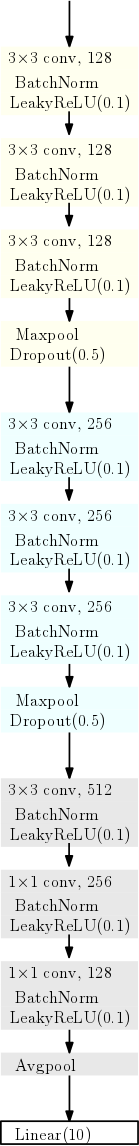
\includegraphics[scale=0.6]{report/figures/net.png}
    \caption{The network architecture: three blocks, each consisting of three convolution layers, and a linear layer for classification.}
    \label{fig:net}
\end{figure}

\onecolumn

\begin{table}
    \centering
    \begin{tabular}{|r|c|c|c|c|}
    \hline
                    & \multicolumn{4}{|c|}{StepLR (step size=30)}            \\ \hline
    momentum        & \multicolumn{2}{|c|}{0.9} & \multicolumn{2}{|c|}{0.95}\\ \hline
    weight decay    & $1e^{-3}$ & $1e^{-4}$     & $1e^{-3}$ & $1e^{-4}$     \\ \hline
    accuracy        & $49.73\%$ & $49.80\%$     & $49.01\%$ & $ 48.85\%$    \\ \hline
    \end{tabular}
    
    \bigskip
    \begin{tabular}{|r|c|c|c|c|}
    \hline
                    & \multicolumn{4}{|c|}{CosineAnnealingLR ($t_{max}$=100)}            \\ \hline
    momentum        & \multicolumn{2}{|c|}{0.9} & \multicolumn{2}{|c|}{0.95}\\ \hline
    weight decay    & $1e^{-3}$ & $1e^{-4}$     & $1e^{-3}$ & $1e^{-4}$     \\ \hline
    accuracy        & $51.16\%$ & $50.01\%$     & $51.62\%$ & $50.48\%$    \\ \hline
    \end{tabular}
        
    \bigskip
    \begin{tabular}{|r|c|c|c|c|}
    \hline
                    & \multicolumn{4}{|c|}{CosineAnnealingWarmRestarts ($t_0$=10)}            \\ \hline
    momentum        & \multicolumn{2}{|c|}{0.9} & \multicolumn{2}{|c|}{0.95}\\ \hline
    weight decay    & $1e^{-3}$ & $1e^{-4}$     & $1e^{-3}$ & $1e^{-4}$     \\ \hline
    accuracy        & $52.59\%$ & $51.20\%$     & $50.90\%$ & $50.41\%$    \\ \hline
%  lr=0.1           & 50.34\%   %    
    \end{tabular}
    \caption{Evaluation results on our changes to increase the baseline accuracy of our network while training for 100 epochs at learning rate of 0.01. The first table shows accuracy when using the \texttt{StepLR} learning rate scheduler with varying momentum and weight decay, the second one the \texttt{CosineAnnealingLR}, and the third one the \texttt{CosineAnnealingWarmRestarts}. Entries show the average accuracy over five runs.}
    \label{tab:baseexp}
\end{table}{}